\chapter{Introduction}
\label{ch:intro}

Complex insect societies are formed by thousands of individuals, which continously move and interact inside a dark nest. Honey bee colonies are thus organized complex social systems, which form a collective intelligence. Observing individual honey bees is therefore vital for understanding collective behavior, decision making and organisation of task within the colony.

The Biorobotics Lab of Freie Universität Berlin developed technologies to track all individuals of a complete honey bee (apis mellifera) colony. Conventional approaches usually focus on a small subset of the hive life, whether this regards time, space, or animal identity~\cite{wario2015automatic}[TODO: change sentence]. All individuals of a colony have been marked on their thorax using circular tags (figure~\ref{fig:markers}). Spatial information for each bee is then recorded for a peroid of nine weeks.


\begin{figure}[htb]
	\centering
	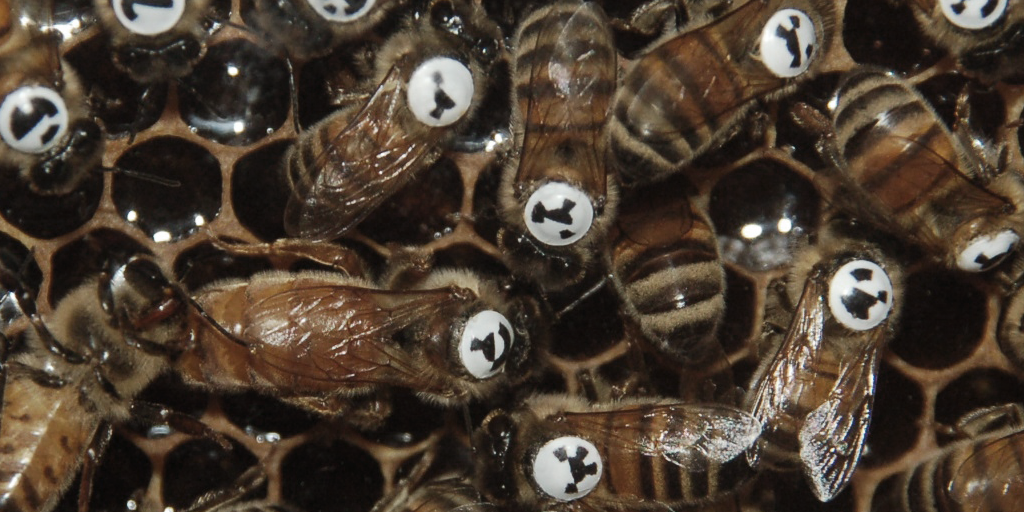
\includegraphics[width=1.0\textwidth]{Figures/markers}
	\caption{Tagged bees inside the hive.}
	\label{fig:markers}
\end{figure}

\section{Motivation}

Most of the studies analysing behaviour of insects colonies only use a small amount of individually labeled animals, a short observation period, and usually manually detect interaction between animals looking at the videos. data~\cite{quevillon2015social}[TODO: more references]. Here it is done in a more inclusive way, all animals, long term observation, automatic detection of individuals.

\section{Research Goal}

Starting off with creating worker-worker interaction networks using spatial proximity as a proxy for interactions between bees.

Answering the following questions:

(1) Is it possible to infer networks with the provided data dataset? (challenges and limitations)\\

(2) Welche Eigenschaften haben diese Netzwerke? Was sind das für Netzwerke? (Netzwerkklasse: ziemlich dichtes (auf keinen fall sparse) Netzwerk, ungerichtetes, gewichtetes Netzwerk (höhres Gewicht, engere Benziehung). no power law degree distribution, daher keine Hubs, sehr geringer Diameter, daher small-world property, small clustering coefficient and giant component.\\

(3) Gibt es in diesen Netzwerken Communities?\\

(4) Wie sind diese charakterisiert? (machen die Sinn) spiegeln die das wieder was man bisher über Bienen weiß? (Alter und Aufenthaltsort)\\

(5) Wie entwicklen sich die Communities über die Zeit?\\
über einen Zeitraum von X tagen (y tage) bleiben die zwei Gruppen erhalten und auch altersverteilung bleibt signifikant verschieden.\\
-> stabilität nachgewiesen?\\
für XY einfach plotten\\

(6) Wie ändern sich die Mitglieder der Communities über die Zeit?\\


\section{Methodology}

Network Science Approach.

\section{Outline}
[TODO]